\subsection{\acs*{cadx}: Classification} \label{subsec:chp3:img-clas:CADX-clas}

%\subsubsection{Classifier} \label{subsubsec:chp3:img-clas:CADX-clas:clas}

\begin{table}
  \caption{Overview of the classifiers used in \acs*{cad} systems.}
  \scriptsize
  \begin{tabularx}{\textwidth}{l >{\raggedleft\arraybackslash}X@{}}
    \toprule
    \textbf{Classifier} & \textbf{References} \\
    \midrule
    \textbf{Rule-based method:} & \cite{Lv2009,Puech2009} \\ \\ [-1.5ex]
    \textbf{Clustering methods:} & \\
    \quad $k$-means clustering & \cite{Tiwari2007,Tiwari2008,Tiwari2009} \\
    \quad \acs{knn} & \cite{Litjens2012,Niaf2011,Niaf2012,rampun2016computerb} \\ \\ [-1.5ex]
    \textbf{Linear model classifiers:} & \\
    \quad \acs{lda} & \cite{Antic2013,Chan2003,Litjens2014,Niaf2011,Niaf2012,Vos2012} \\
    \quad Logistic regression & \cite{Kelm2007,Langer2009,lehaire2014computer,rampun2015computer} \\ \\ [-1.5ex]
    \textbf{Non-linear classifier:} & \\
    \quad \acs{qda} & \cite{Viswanath2012} \\ \\ [-1.5ex]
    \textbf{Probabilistic classifier:} & \\
    \quad Naive Bayes & \cite{Giannini2013,Mazzetti2011,Niaf2011,Niaf2012,cameron2014multiparametric,cameron2016maps,rampun2015classifying,rampun2016computerb,rampun2015computer,rampun2016computer} \\ \\ [-1.5ex]
    \textbf{Ensemble learning classifiers:} & \\
    \quad AdaBoost & \cite{Litjens2014,Lopes2011} \\
    \quad \acs*{rf} & \cite{Kelm2007,Litjens2014,Tiwari2012,Tiwari2013,Viswanath2009,trigui2017automatic,trigui2016classification,samarasinghe2016semi,rampun2015classifying,rampun2016computerb,rampun2015computer,rampun2016computer} \\
    \quad Probabilistic boosting tree & \cite{Tiwari2009,Tiwari2010,Tiwari2012} \\ \\ [-1.5ex]
    \textbf{Kernel method:} & \\
    \quad Gaussian processes & \cite{Kelm2007} \\ \\ [-1.5ex]
    \textbf{Sparse kernel methods:} & \\
    \quad \acs{svm} & \cite{Artan2009,Artan2010,Chan2003,Litjens2011,Litjens2012,Liu2013,Lopes2011,Niaf2011,Niaf2012,Ozer2009,Ozer2010,Parfait2012,Peng2013,Sung2011,Tiwari2012,Vos2008,Vos2008a,Vos2010,Vos2012,giannini2015fully,trigui2017automatic,lehaire2014computer,khalvati2015automated,chung2015prostate} \\
    \quad \acs{rvm} & \cite{Ozer2009,Ozer2010} \\ \\ [-1.5ex]
    \textbf{Neural network:} & \\ 
    \quad Multiple layer perceptron & \cite{Matulewicz2013,Parfait2012,trigui2017automatic,trigui2016classification,rampun2016computer} \\
    \quad Probabilistic neural network & \cite{Ampeliotis2007,Ampeliotis2008,Viswanath2011} \\ \\ [-1.5ex]
    \textbf{Graphical model classifiers:} & \\
    \quad Markov random field & \cite{Liu2009,Ozer2010} \\
    \quad Conditional random field & \cite{Artan2009,Artan2010,chung2015prostate} \\
    \bottomrule
  \end{tabularx}
\label{tab:class}
\end{table}

Once the feature vector has been extracted and eventually the complexity reduced, it is possible to make a decision and classify this feature vector to belong to \ac{cap} or healthy tissue.
Classification methods used in \ac{cad} system to distinguish these two classes are summarized in \acs{tab}~\ref{tab:class}.
A full review of classification methods used in pattern recognition is available found in~\cite{Bishop2006}.

\paragraph{Rule-based method}
\citeauthor{Lv2009} make use of a decision stump classifier to distinguish \ac{cap} and healthy classes~\cite{Lv2009}. 
\citeauthor{Puech2009} detect \ac{cap} by implementing a given set of rules and scores based on a medical support approach~\cite{Puech2009}.
During the testing, the feature vector go through these different rules, and a final score is computed resulting to a final decision.

\paragraph{Clustering methods}
\acf{knn} is one of the simplest supervised machine learning classification methods.
In this method, a new unlabelled vector is assigned to the most represented class from its $k$ nearest-neighbours in the feature space.
The parameter $k$ is usually an odd number in order to avoid any tie case.
\ac{knn} has been one of the method used in~\cite{Niaf2011,Niaf2012,rampun2016computerb} mainly to make a comparison with different machine learning techniques.
\citeauthor{Litjens2012} used this method to roughly detect potential \ac{cap} voxels before performing a region-based classification~\cite{Litjens2012}.

The $k$-means algorithm is an unsupervised clustering method in which the data is partitioned into $k$ clusters in an iterative manner.
First, $k$ random centroids are defined in the feature space and each data point is assigned to the nearest centroid.
Then, the centroid position for each cluster is updated by computing the mean of all the samples belonging to this particular cluster.
Both assignment and updating are repeated until the centroids are stable.
The number of clusters $k$ is usually defined as the number of classes.
This algorithm can also be used for ``on-line'' learning.
In case that new data has to be incorporated, the initial centroid positions correspond to the results of a previous $k$-means training and is followed by the assignment-updating stage previously explained.
\citeauthor{Tiwari2009} used $k$-means in an iterative procedure~\cite{Tiwari2007,Tiwari2009}.
Three clusters have been defined corresponding to \ac{cap}, healthy, and non-prostate.
$k$-means is repeatedly applied and at each iteration, the voxels corresponding to the largest cluster are excluded under the assumption that it is assigned to ``non-prostate'' cluster.
The algorithm stopped when the number of voxels in all remaining clusters are smaller than a given threshold.
\citeauthor{Tiwari2008} and \citeauthor{Viswanath2008a} used $k$-means in a repetitive manner in order to be less sensitive to the centroids initialization~\cite{Viswanath2008,Viswanath2008a,Tiwari2008}.
Thus, $k$ clusters are generated $T$ times and the final assignment is performed by majority voting using a co-association matrix as proposed in~\cite{Fred2005}.

\paragraph{Linear model classifiers}
\Acf{lda} is used as a classification method in which the optimal linear separation between 2 classes is found by maximizing the inter-class variance and minimizing the intra-class variance~\cite{Friedman1989}.
The linear discriminant function is defined as:
\begin{equation}
	\delta_{k}(\mathbf{x}_i) = \mathbf{x}_i^{\text{T}} \Sigma^{-1} \mu_k - \frac{1}{2} \mu_{k}^{\text{T}} \Sigma^{-1} \mu_k + \log (\pi_k) \ ,
	\label{eq:ldafun}
\end{equation}

\noindent where $\mathbf{x}_i$ is an unlabelled feature vector, $\Sigma$ is the covariance matrix of the training data, $\mu_k$ is the mean vector of the class $k$, and $\pi_k$ is the prior probability of class $k$.
To perform the classification, a sample $\mathbf{x}_i$ is assigned to the class which maximizes the discriminant function as in \acs{eq}\,\eqref{eq:ldaclass}.
\begin{equation}
	C(\mathbf{x}_i) = \argmax_k \delta_k(\mathbf{x}_i) \ .
	\label{eq:ldaclass}
\end{equation}
\Ac{lda} has been used in~\cite{Antic2013,Chan2003,Niaf2011,Niaf2012,Vos2012}.

%covariance matrix $\Sigma_k$ specific at each class is computed.
%used \ac{lda} to classify their feature vectors defining two classes \ac{cap} \textit{versus} healthy

Logistic regression is also used to perform binary classification and provides the probability of an observation to belong to a class.
The posterior probability of one of the classes, $c_1$ is written as:
\begin{equation}
	p(c_1|\mathbf{x}_i) = \frac{1}{1+\exp(-\mathbf{w}^{\text{T}}\mathbf{x}_i)} \ ,
	\label{eq:postprlr}
\end{equation}

\noindent with $p(c_2|\mathbf{x}_i) = 1 - p(c_1|\mathbf{x}_i)$ and where $\mathbf{w}$ is the vector of the regression parameters allowing to obtain a linear combination of the input feature vector $\mathbf{x}_i$.
Thus, an unlabelled observation $\mathbf{x}_i$ is assigned to the class which maximizes the posterior probability as shown in \acs{eq}\,\eqref{eq:posprobreg}.

\begin{equation}
	C(\mathbf{x}_i) = \argmax_k p(C=k|\mathbf{x}_i) \ .
	\label{eq:posprobreg}
\end{equation}

From \acs{eq}\,\eqref{eq:postprlr}, one can see that the key to classification using logistic regression model is to infer the set of parameters $\mathbf{w}$ through a learning stage using a training set.
This vector of parameters $\mathbf{w}$ is inferred by estimating the maximum likelihood.
This step is performed through an optimization scheme, using a quasi-Newton method~\cite{Byrd1995}, which seeks in an iterative manner for the local minimum in the derivative of \acs{eq}\,\eqref{eq:postprlr}.
This method has been used to create a linear probabilistic model in~\cite{Kelm2007,Puech2009,lehaire2014computer,rampun2015computer}.

\paragraph{Non-linear model classifier}
\citeauthor{Viswanath2012} used \acf{qda} instead of \ac{lda}~\cite{Viswanath2012}.
Unlike in \ac{lda} in which one assumes that the class covariance matrix $\Sigma$ is identical for all classes, a covariance matrix $\Sigma_k$ specific to each class is computed.
Thus, \acs{eq}\,\eqref{eq:ldafun} becomes:
\begin{equation}
	\delta_{k}(\mathbf{x}_i) = \mathbf{x}_i^{\text{T}} \Sigma_{k}^{-1} \mu_k - \frac{1}{2} \mu_{k}^{\text{T}} \Sigma_{k}^{-1} \mu_k + \log (\pi_k) \ .
	\label{eq:qdafun}
\end{equation}

The classification scheme in the case of the \ac{qda} is identical to \acs{eq}\,\eqref{eq:ldaclass}.

\paragraph{Probabilistic classifiers}
The most commonly used classifier is the naive Bayes classifier which is a probabilistic classifier assuming independence between each feature dimension~\cite{Rish2001}.
This classifier is based on Bayes' theorem:

\begin{equation}
	p(C=k|\mathbf{x}) = \frac{p(C)p(\mathbf{x}|C)}{p(\mathbf{x})} \ ,
	\label{eq:bayth}
\end{equation}

\noindent where $p(C=k|\mathbf{x})$ is the posterior probability, $p(C)$ is the prior probability, $p(\mathbf{x}|C)$ is the likelihood, and $p(\mathbf{x})$ is the evidence. 
However, the evidence term is usually discarded since it is not class dependent and plays the role of a normalization term.
Hence, in a classification scheme, an unlabelled observation is classified to the class which maximizes the posterior probability as:

\begin{eqnarray}
	C(\mathbf{x}_i) & = & \argmax_k p(C=k|\mathbf{x}_i) \ , \label{eq:maxbay} \\
	p(C=k|\mathbf{x}_i) & = & p(C=k) \prod_{j=1}^{n} p(x_{ij},|C=k) \ , \label{eq:postbay}
\end{eqnarray}

\noindent where $d$ is the number of dimensions of the feature vector $\mathbf{x}_i = \{x_{i1},\cdots,x_{id}\}$.
Usually, a model includes both the prior and likelihood probabilities and it is common to use an equal prior probability for each class or eventually a value based on the relative frequency derived from the training set.
Regarding the likelihood probability, it is common to choose a Gaussian distribution to characterize each class.
Thus, each class is characterized by two parameters: (i) the mean and (ii) the standard deviation.
These parameters are inferred from the training set by using the \ac{mle} approach.
The naive Bayes classifier has been used in~\cite{Giannini2013,Mazzetti2011,Niaf2011,Niaf2012,Niaf2012,cameron2014multiparametric,cameron2016maps,rampun2015classifying,rampun2016computerb,rampun2015computer,rampun2016computer}.

\paragraph{Ensemble learning classifiers}
AdaBoost is an adaptive method based on an ensemble learning method and initially proposed in~\cite{Freund1997}. 
AdaBoost linearly combines several weak learners resulting into a final strong classifier.
A weak learner is defined as a classification method performing slightly better than a random classifier.
Popular choices regarding the weak learner classifiers are: decision stump or decision tree learners such as \ac{id3}~\cite{Quinlan1986}, C4.5~\cite{Quinlan1993}, and \ac{cart}~\cite{Breiman1984}.

AdaBoost is considered as an adaptive method in the way that the weak learners are selected.
The selection is performed in an iterative manner.
At each iteration $t$, the weak learner selected $h_t$ corresponds to the one minimizing the classification error on a distribution of weights $D_t$, that is associated with the training samples.
Each weak learner is assigned a weight $\alpha_t$ as:

\begin{equation}
	\alpha_t = \frac{1}{2} \ln \frac{1 - \epsilon_t}{\epsilon_t} \ ,
	\label{eq:wclssada}
\end{equation}

\noindent where $\epsilon_t$ corresponds to the classification error rate of the weak learner on the distribution of weight $D_t$.

Before performing a new iteration, the distribution of weights $D_t$ is updated such that the weights associated with the misclassified samples by $h_t$ increase and the weights of well classified samples decrease as shown in \acs{eq}\,\eqref{eq:rewada}.

\begin{equation}
	D_{t+1}(i) = \frac{ D_t(i) \exp \left( -\alpha_t y_i h_{t}(\mathbf{x}_{i} ) \right) }{ Z_t  } \ ,
	\label{eq:rewada} 
\end{equation}

\noindent where $\mathbf{x}_i$ is the $i^{\text{th}}$ sample corresponding to class $y_i$ and $Z_t$ is a normalization factor forcing $D_{t+1}$ to be a probability distribution. 
This procedure allows to select a weak learner at the next iteration $t+1$ which will classify in priority the previous misclassified samples. 
Thus, after $T$ iterations, the final strong classifier corresponds to the linear combination of the weak learners selected and the classification is performed such that:

\begin{equation}
	C(\mathbf{x}_i) = \sign \left( \sum_{t=1}^{T} \alpha_t h_t(\mathbf{x}_i) \right) \ .
	\label{eq:strclaada}
\end{equation}

\citeauthor{Lopes2011} make use of the AdaBoost classifier to perform their classification~\cite{Lopes2011} while \citeauthor{Litjens2014} used the GentleBoost variant~\cite{Friedman1998} which provides a modification of the function affecting the weight at each weak classifier~\cite{Litjens2014}.

\ac{rf} is a classification method which is based on creating an ensemble of decision trees and was introduced in~\cite{Breiman2001}.
In the learning stage, multiple decision tree learners~\cite{Breiman1984} are trained.
However, each decision tree is trained using a different dataset.
Each of these datasets corresponds to a bootstrap sample generated by randomly choosing $n$ samples with replacement from the initially $N$ samples available~\cite{Efron1979}.
Then, randomization is also part of the decision tree growth.
At each node of the decision tree, from the bootstrap sample of $D$ dimensions, a number of $d \ll D$ dimensions will be randomly selected.
Finally, the $d^{\text{th}}$ dimension in which the classification error is minimum is used.
This best ``split'' classifier is often evaluated using \ac{mi} or Gini index.
Finally, each tree is grown as much as possible without using any pruning procedure.
In the prediction stage, the unlabelled sample is introduced in each tree and each of them assign a class.
Finally, it is common to use a majority voting approach to choose the final class label.
The \ac{rf} classifier has been used in~\cite{Kelm2007,Litjens2014,Tiwari2012,Tiwari2013,Viswanath2009,trigui2017automatic,trigui2016classification,samarasinghe2016semi,rampun2015classifying,rampun2016computerb,rampun2015computer,rampun2016computer}.

\begin{figure}
\centering
	\begin{tikzpicture}
    [level distance=1.75cm,sibling distance=1.5cm,scale=.95,every node/.style={scale=0.95}, 
   edge from parent path={(\tikzparentnode) -- (\tikzchildnode)}]
	\Tree [.\node (foo) {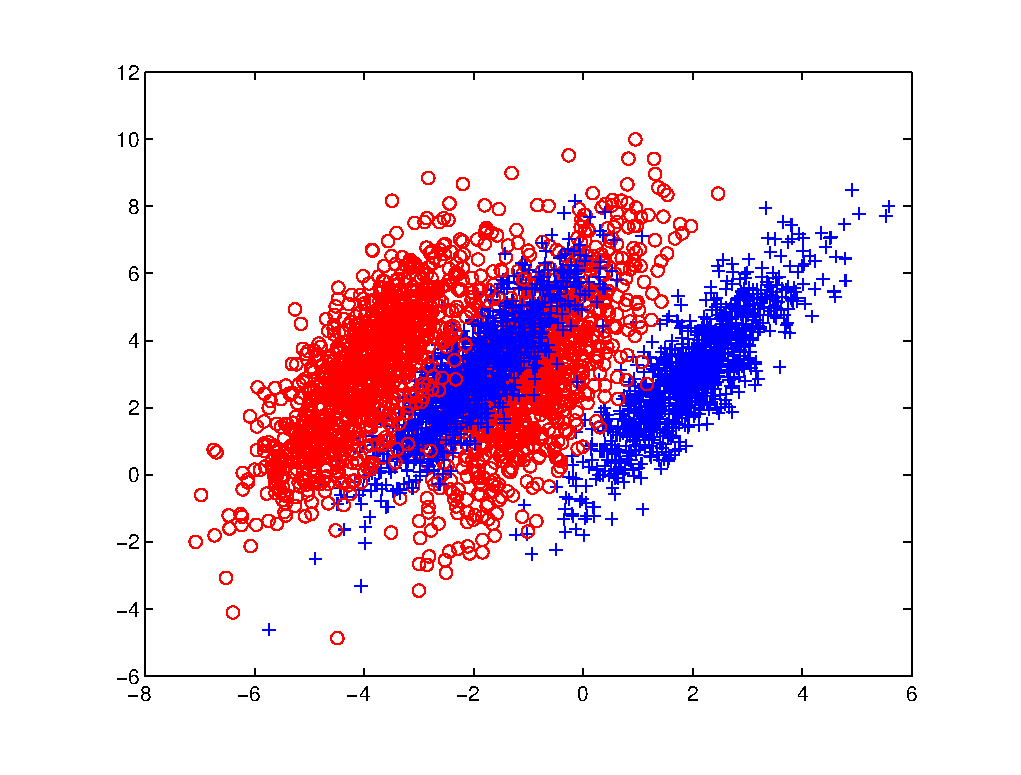
\includegraphics[width=2cm]{3_review/figures/classification/pbt-simulation/pbt_tree_1.eps}}; 
    \edge node[auto=right] {};
    [.\node{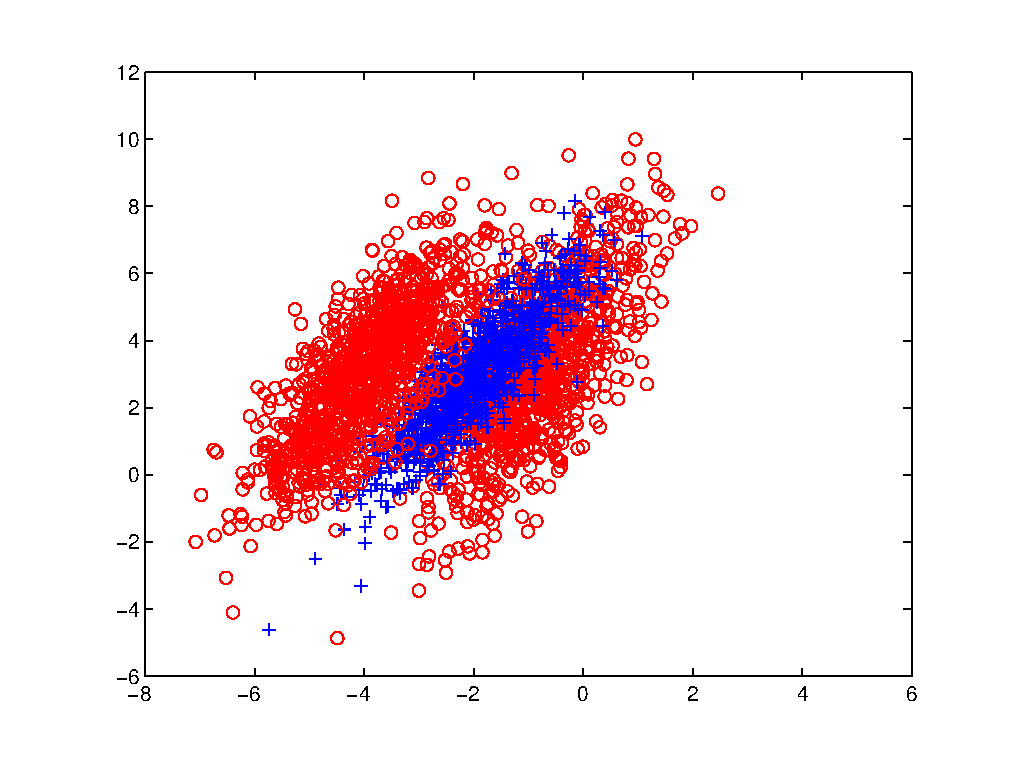
\includegraphics[width=2cm]{3_review/figures/classification/pbt-simulation/pbt_tree_2_1.eps}};
      \edge node[auto=right] {};  
      [.\node{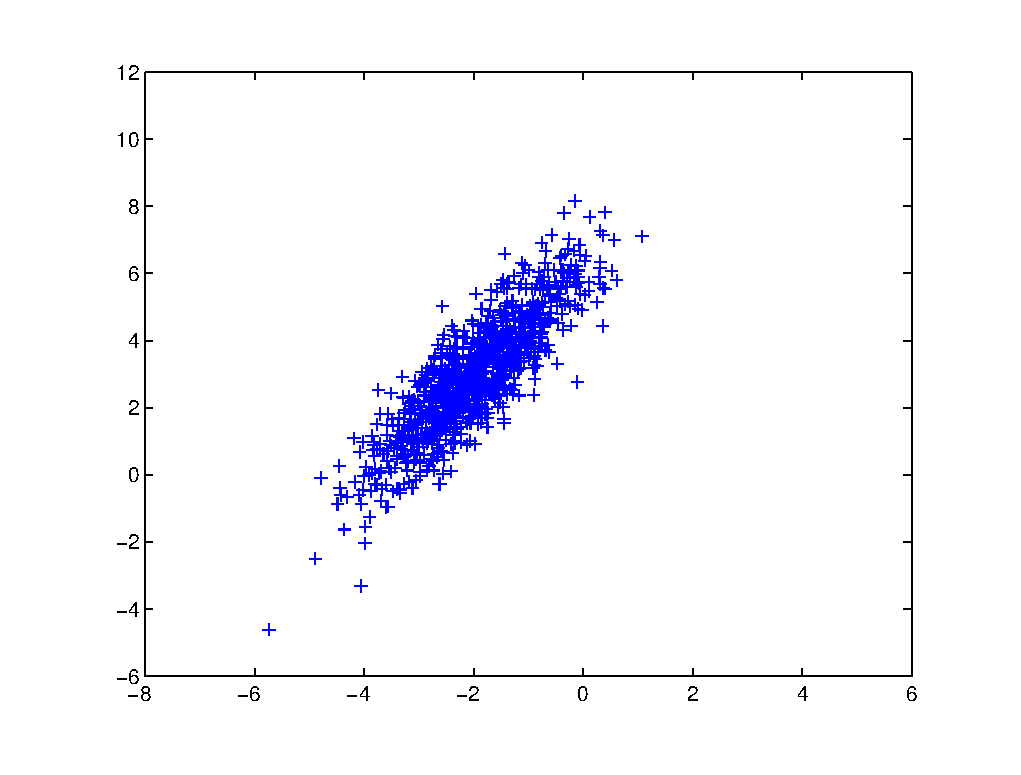
\includegraphics[width=2cm]{3_review/figures/classification/pbt-simulation/pbt_tree_3_2.eps}}; ]
      \edge node[auto=left] {};  
      [.\node{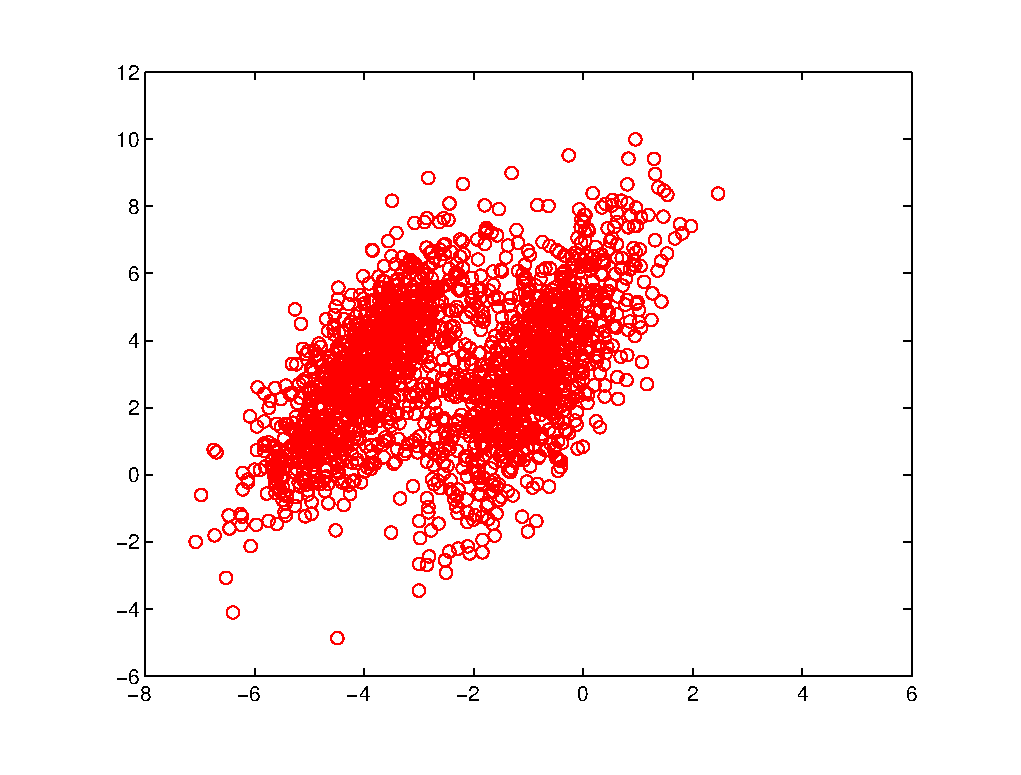
\includegraphics[width=2cm]{3_review/figures/classification/pbt-simulation/pbt_tree_3_1.eps}}; ]
    ]
    \edge node[auto=left] {};
    [.\node{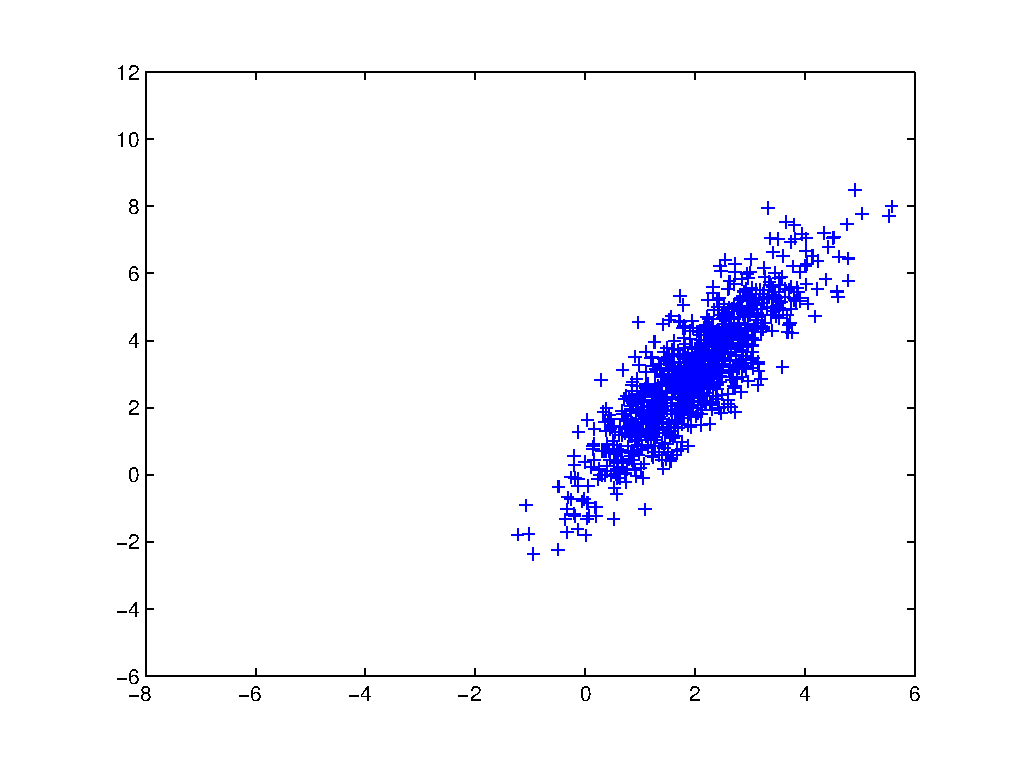
\includegraphics[width=2cm]{3_review/figures/classification/pbt-simulation/pbt_tree_2_2.eps}};
    ]
    ];
	\end{tikzpicture}
\caption[Representation of the probabilistic boosting-tree.]{Representation of the capabilities of the probabilistic boosting-tree algorithm to split at each node of the tree the positive and negative samples.}
\label{fig:pbtsim}
\end{figure}

Probabilistic boosting-tree is another ensemble learning classifier which shares principles with AdaBoost but using them inside a decision tree~\cite{Tu2005}. 
In the training stage, the probabilistic boosting-tree method grows a decision tree and at each node, a strong classifier is learned in an almost comparable scheme to AdaBoost.
Once the strong learner is trained, the training set is split into two subsets which are used to train the next strong classifiers in the next descending nodes.
Thus, three cases are conceivable to decide in which branch to propagate each sample training $\mathbf{x}_i$:

\begin{itemize}
	\item if $q(+1, \mathbf{x}_i) - \frac{1}{2} > \epsilon$ then $\mathbf{x}_i$ is propagated to the right branch set and a weight $w_i=1$ is assigned. 
	\item if $q(-1, \mathbf{x}_i) - \frac{1}{2} > \epsilon$ then $\mathbf{x}_i$ is propagated to the left branch set and a weight $w_i=1$ is assigned.
	\item else $\mathbf{x}_i$ will be propagated in both branches with $w_i=q(+1, \mathbf{x}_i)$ in the right branch and $w_i=q(-1, \mathbf{x}_i)$ in the left branch.
\end{itemize}

\noindent with $\mathbf{w} = w_i, i=\{1,\cdots,N\}$ corresponding to distribution of weights, $N$ the number of samples as in AdaBoost and $q(\cdot)$ is defined as:

\begin{eqnarray}
	q(+1, \mathbf{x}_i) & = & \frac{\exp(2H(\mathbf{x}_i))}{1+\exp(2H(\mathbf{x}_i))} \ , \label{eq:regada1} \\
	q(-1, \mathbf{x}_i) & = & \frac{\exp(-2H(\mathbf{x}_i))}{1+\exp(-2H(\mathbf{x}_i))} \ . \label{eq:regada2}
\end{eqnarray}

Employing such a scheme tends to divide the data in such a way that positive and negative samples are naturally split as shown in \acs{eq}\,\ref{fig:pbtsim}.
In the classification stage, the unlabelled sample $\mathbf{x}$ is propagated through the tree, where at each node, it is classified by each strong classifier previously learned and where an estimation of the posterior distribution is computed.
The posterior distribution corresponds to the sum of the posterior distribution at each node of the decision tree.
The probabilistic boosting-tree classifier has been used in~\cite{Tiwari2009a,Tiwari2012,Tiwari2010,Viswanath2011}.

\paragraph{Kernel method}
A Gaussian process for classification is a kernel method in which it is assumed that the data can be represented by a single sample from a multivariate Gaussian distribution~\cite{Rasmussen2005}.
In the case of linear logistic regression for classification, the posterior probability is expressed as:
\begin{eqnarray}
	p(y_i|\mathbf{x}_i,\mathbf{w}) & = & \sigma(y_i f(\mathbf{x}_i)) \ , \label{eq:gp1} \\
	f(\mathbf{x}_i) & = & \mathbf{x}_i^{\text{T}} \mathbf{w} \ , \nonumber
\end{eqnarray}

\noindent where $\sigma(\cdot)$ is the logistic function and $\mathbf{w}$ are the parameters vector of the model.
Thus, the classification using Gaussian processes is based on assigning a Gaussian process prior over the function $f(\mathbf{x})$ which is characterized by a mean function $\bar{f}$ and covariance function $K$.
Therefore, in the training stage, the best mean and covariance functions have to be inferred in regard to our training data using a Newton optimization and a Laplacian approximation.
The prediction stage is performed in two stages.
First, for a new observation $\mathbf{x}_*$, the corresponding probability $p(f(\mathbf{x}_*)|f(\mathbf{x}))$ is computed such that:
\begin{eqnarray}
	p(f(\mathbf{x}_*)|f(\mathbf{x})) & = & \mathcal{N}( K_*K^{-1}\bar{f}, K_{**}-K_*(K')^{-1}K_*^{\text{T}} ) \ , \nonumber \\
	K' & = & K + W^{-1} \ , \label{eq:gp2} \\
	W & = & \nabla \nabla \log p(\mathbf{y}|f(\mathbf{x})) \ , \nonumber
\end{eqnarray}

\noindent where $K_{**}$ is the variance of the testing sample $\mathbf{x}_*$, $K_{*}$ is the covariance of training-testing samples $\mathbf{x}$ and $\mathbf{x}_*$.
Then, the function $f(\mathbf{x}_*)$ is squashed using the sigmoid function and the probability of the class membership is defined such that:

\begin{equation}
	C(\mathbf{x}_*) = \sigma\left( \frac{\bar{f}(\mathbf{x_*})}{\sqrt{1+var(f(\mathbf{x}_*))}} \right) \ .
	\label{eq:gp3}
\end{equation}

Only \citeauthor{Kelm2007} used Gaussian process for classification of \ac{mrsi} data~\cite{Kelm2007}.

\paragraph{Sparse kernel methods}
In a classification scheme using Gaussian processes, when a prediction is performed, the whole training data are used to assign a label to the new observations.
That is why this method is also called kernel method.
Sparse kernel category is composed of methods which rely only on a few labelled observations of the training set to assign the label of new observations~\cite{Bishop2006}.

\Acf{svm} is a sparse kernel method aiming at finding the best linear hyper-plane --- non-linear separation is discussed further --- which separates 2 classes such that the margin between the two classes is maximized~\cite{Vapnik1963}.
The margin is in fact the region defined by 2 hyper-planes splitting the 2 classes, such that there is no points lying in between.
The distance between these 2 hyper-planes is equal to $\frac{2}{\|\mathbf{w}\|}$ where $\mathbf{w}$ is the normal vector of the hyper-plane splitting the classes.
Thus, maximizing the margin is equivalent to minimizing the norm $\|\mathbf{w}\|$.
Hence, this problem is solved by an optimization approach and formalized as:

\begin{equation}
\begin{aligned}
& \argmin_{\mathbf{w}}
& & \frac{1}{2} \| \mathbf{w}^2\| \ , \\
& \text{subject to}
& & y_i(\mathbf{w}.\mathbf{x}_i - b) \geq 1, \; i = \{ 1, \ldots, N \} \ ,
\end{aligned}
\label{eq:svm1}
\end{equation}

\noindent where $\mathbf{x}_i$ is a training sample with is corresponding class label $y_i$.
From \acs{eq}\,\eqref{eq:svm1}, it is important to notice that only few points from the set of $N$ points are selected which later define the hyper-plane.
This constraint is imposed in the optimization problem using Lagrange multipliers $\boldsymbol{\alpha}$.
All points which are not lying on the margin are assigned a corresponding $\alpha_i = 0$, which is formalized as \acs{eq}\,\eqref{eq:svm2}.

\begin{equation}
	\arg\min_{\mathbf{w},b } \max_{\boldsymbol{\alpha}\geq 0 } \left\{ \frac{1}{2}\|\mathbf{w}\|^2 - \sum_{i=1}^{n}{\alpha_i[y_i(\mathbf{w}\cdot \mathbf{x_i} - b)-1]} \right\} \ .
	\label{eq:svm2}
\end{equation}

The different parameters are inferred using quadratic programming.
This version of \ac{svm} is known as hard-margin since no points can lie in the margin area.
However, it is highly probable not to find any hyper-plane splitting the classes such as specified previously.
Thus, a soft-margin optimization approach has been proposed~\cite{Cortes1995}, where points have the possibility to lie on the margin but at the cost of a penalty $\xi_i$ which is minimized in the optimization process such that:

\begin{equation}
\small
\arg\min_{\mathbf{w},\mathbf{\xi}, b } \max_{\boldsymbol{\alpha},\boldsymbol{\beta} } \left\{ \frac{1}{2}\|\mathbf{w}\|^2+C \sum_{i=1}^n \xi_i - \sum_{i=1}^{n}{\alpha_i[y_i(\mathbf{w}\cdot \mathbf{x_i} - b) -1 + \xi_i]} - \sum_{i=1}^{n} \beta_i \xi_i \right\} \ .
\end{equation}

The decision to assign the label to a new observation $\mathbf{x}_i$ is taken such that:

\begin{equation}
	C(\mathbf{x}_i) = \sign \left( \sum_{n=1}^{N} \alpha_n (\mathbf{x}_n . \mathbf{x}_i) + b_0 \right) \ ,
	\label{eq:svmdec} 
\end{equation}

\noindent where $\mathbf{x}_n|n=\{1,\cdots,S\}$, $S$ being the support vectors.

\ac{svm} can also be used as a non-linear classifier by performing a Kernel trick~\cite{Boser1992}.
The original data $\mathbf{x}$ is projected to a high-dimensional space in which it is assumed that a linear hyper-plane splits the 2 classes.
Different kernels are popular such as the \ac{rbf} kernel, polynomial kernels, or sigmoid kernel.
In \ac{cad} for \ac{cap} systems, \ac{svm} is the most popular classification method and has been used in a multitude of research works~\cite{Artan2009,Artan2010,Chan2003,Litjens2011,Litjens2012,Liu2013,Lopes2011,Niaf2011,Niaf2012,Ozer2009,Ozer2010,Parfait2012,Peng2013,Sung2011,Tiwari2012,Vos2008,Vos2008a,Vos2010,Vos2012,giannini2015fully,trigui2017automatic,lehaire2014computer,khalvati2015automated,chung2015prostate}.

\Acf{rvm} is a sparse version of Gaussian process previously presented, proposed in~\cite{Tipping2001}.
\ac{rvm} is identical to a Gaussian process with the following covariance function~\cite{Quinonero-Candela2002}:

\begin{equation}
	K_{RVM}(\mathbf{x}_p,\mathbf{x}_q) = \sum_{j=1}^{M} \frac{1}{\alpha_j} \Phi_j ( \mathbf{x}_p ) \Phi_j ( \mathbf{x}_q ) \ ,
 	\label{eq:rvm}
\end{equation}

\noindent where $\phi(\cdot)$ is a Gaussian basis function, $\mathbf{x}_i|i=\{1,\cdots,N\}$ are the $N$ training points, and $\boldsymbol{\alpha}$ are the weights vector.
As mentioned in~\cite{Quinonero-Candela2002}, the sparsity regarding the relevance vector arises if $j \alpha_j^{-1} = 0$.
The set of weights $\boldsymbol{\alpha}$ is inferred using the expectation maximization algorithm.
\citeauthor{Ozer2010} usde of \ac{rvm} and make a comparison with \ac{svm} for the task of \ac{cap} detection~\cite{Ozer2009,Ozer2010}.

\paragraph{Neural network} 
Multilayer perceptron is a feed-forward neural networks considered as the most successful model of this kind in pattern recognition~\cite{Bishop2006}.
The most well known model used is based on 2 layers where a prediction of an observation is computed as:

\begin{equation}
	C(\mathbf{x}_n,w_{ij}^{(1)},w_{kj}^{(2)}) = \sigma \left[ \sum_{j=0}^{M} w_{kj}^{(2)} \  h \left( \sum_{i=0}^{D} w_{ij}^{(1)} x_{in} \right) \right] \ ,
	\label{eq:annmlp}
\end{equation}

\noindent where $h(\cdot)$ and $\sigma(\cdot)$ are 2 activation functions usually non-linear, $w_{ij}^{(1)}$ and $ w_{kj}^{(2)}$ are the weights associated with the linear combination with the input feature $\mathbf{x}_n$ and the hidden unit.

\begin{figure}
\centering
\def\layersep{3cm}
\begin{tikzpicture}[shorten >=1pt,draw=black!50, node distance=\layersep]
    \tikzstyle{every pin edge}=[<-,shorten <=1pt]
    \tikzstyle{neuron}=[circle,fill=black!25,minimum size=17pt,inner sep=0pt]
    \tikzstyle{input neuron}=[neuron, fill=green!20];
    \tikzstyle{output neuron}=[neuron, fill=red!80];
    \tikzstyle{hidden neuron}=[neuron, fill=blue!40];
    \tikzstyle{annot} = [text width=4em, text centered]

    % Draw the input layer nodes
    \foreach \name / \y in {1,...,3}
    % This is the same as writing \foreach \name / \y in {1/1,2/2,3/3,4/4}
        \node[input neuron] (I-\name) at (0,-\y) {\tiny $x_{ \y n }$};
        
   \node[input neuron] (I-4) at (0,-4.5) {\tiny $x_{in}$};
   \draw[dashed,draw=black!50] (I-3) -- (I-4);

    % Draw the hidden layer nodes
    \foreach \name / \y in {1,...,4}
        \path[yshift=0.5cm]
            node[hidden neuron] (H-\name) at (\layersep,-\y cm) {\tiny $h_{ \y }\left(\sum \cdot \right)$};
            
    \node[hidden neuron] (H-5) at (\layersep,-5.5 cm) {\tiny $h_{j}\left(\sum \cdot \right)$};
    \draw[dashed,draw=black!50] (H-4) -- (H-5);

    % Draw the output layer node
    	\node[output neuron,pin={[pin edge={->}]right:$C_{0}$}, right of=H-2] (O-1) {\tiny $\sigma\left(\sum \cdot \right)$};
    	\node[output neuron,pin={[pin edge={->}]right:$C_{1}$}, right of=H-4] (O-2) {\tiny $\sigma\left(\sum \cdot \right)$};

    % Connect every node in the input layer with every node in the
    % hidden layer.
    \foreach \source in {1,...,4}
        \foreach \dest in {1,...,5}
        		\draw[shorten >=1pt,->,draw=black!50] (I-\source)  -- (H-\dest);
            %\path (I-\source) edge (H-\dest);
    
    % Draw the annotation for the weight for the first and last connections       
    \draw[shorten >=1pt,->,draw=black!50] (I-1) -- (H-1) node [midway, above] (w111) {\scriptsize $w_{11}^{(1)}$};
    \draw[shorten >=1pt,->,draw=black!50] (I-4) -- (H-5) node [midway, below] (w145) {\scriptsize $w_{ij}^{(1)}$};

    % Connect every node in the hidden layer with the output layer
    \foreach \source in {1,...,5}
    		\foreach \dest in {1,...,2}
        		\draw[shorten >=1pt,->,draw=black!50] (H-\source)  -- (O-\dest);
        %\path (H-\source) edge (O);
        
    % Draw the annotation for the weight for the first and last connections       
    \draw[shorten >=1pt,->,draw=black!50] (H-1) -- (O-1) node [midway, above] (w211) {\scriptsize $w_{11}^{(2)}$};
    \draw[shorten >=1pt,->,draw=black!50] (H-5) -- (O-2) node [midway, below] (w251) {\scriptsize $w_{kj}^{(2)}$};

    % Annotate the layers
    \node[annot,above of=H-1, node distance=1cm] (hl) {\footnotesize Hidden layer};
    \node[annot,left of=hl] {\footnotesize Input layer};
    \node[annot,right of=hl] {\footnotesize Output layer};
\end{tikzpicture}
\caption{Representation of a neural network of the multilayer perceptron family.}
\label{fig:mlp}
\end{figure}


A graphical representation of this network is presented in \acs{eq}\,\ref{fig:mlp}.
Relating \acs{fig}\,\ref{fig:mlp} with \acs{eq}\,\eqref{eq:annmlp}, it can be noted that this network is composed of some successive non-linear mapping of the input data.
First, a linear combination of the input vector $\mathbf{x}_n$ is mapped into some hidden units through a set of weights $w_{ij}^{(1)}$.
This combination becomes non-linear by the use of the activation function $h(\cdot)$ which is usually chosen to be a sigmoid function.
Then, the output of the networks consists of a linear combination of the hidden units and the set of weights $w_{kj}^{(2)}$.
This combination is also mapped non-linearly using an activation function $\sigma(\cdot)$ which is usually a logistic function.
Thus, the training of such a network resides in finding the best weights $w_{ij}^{(1)}$ and $ w_{kj}^{(2)}$ which model the best the training data.
The error of this model is computed as:

\begin{equation}
	E(w_{ij}^{(1)},w_{kj}^{(2)}) = \frac{1}{2} \sum_{n=1}^{N} \left( C(\mathbf{x}_n,w_{ij}^{(1)},w_{kj}^{(2)}) - y(\mathbf{x}_n) \right) ^{2} \ ,
	\label{eq:mlpcost}
\end{equation}

\noindent where $\mathbf{x}_n|n=\{1,\cdots,N\}$ are the $N$ training vectors with their corresponding class label $y(\mathbf{x}_n)$.

Therefore, the best set of weights is inferred in an optimization framework where the error $E(\cdot)$ needs to be minimized.
This optimization is performed using a gradient descent method where the derivative of \acs{eq}\,\eqref{eq:mlpcost} is computed using the back-propagation algorithm proposed by~\cite{Rumelhart1988}.
This type of network has been used multiple times~\cite{Matulewicz2013,Parfait2012,trigui2017automatic,trigui2016classification,rampun2016computer}.

\begin{figure}
\centering
\def\layersep{3cm}
\def\finallayersep{2.2cm}
\begin{tikzpicture}[shorten >=1pt,draw=black!50, node distance=\layersep]
    \tikzstyle{every pin edge}=[<-,shorten <=1pt]
    \tikzstyle{neuron}=[circle,fill=black!25,minimum size=20pt,inner sep=0pt]
    \tikzstyle{input neuron}=[neuron, fill=green!20];
    \tikzstyle{output neuron}=[neuron, fill=red!80];
    \tikzstyle{hidden neuron}=[neuron, fill=blue!20];
    \tikzstyle{summation neuron}=[neuron, fill=blue!40];
    \tikzstyle{annot} = [text width=4em, text centered]

    % Draw the input layer nodes
    \foreach \name / \y in {1,...,3}
    % This is the same as writing \foreach \name / \y in {1/1,2/2,3/3,4/4}
        \node[input neuron] (I-\name) at (0,-\y-1) {\tiny $x_{ \y n }$};
        
   \node[input neuron] (I-4) at (0,-5.5) {\tiny $x_{in}$};
   \draw[dashed,draw=black!50] (I-3) -- (I-4);
   
   % Draw the pattern layer
   \node[hidden neuron] (H-1) at (\layersep,0 cm) {\tiny $h_{11}\left( \cdot \right)$};
   \node[hidden neuron] (H-2) at (\layersep,-1 cm) {\tiny $h_{21}\left( \cdot \right)$};
   \node[hidden neuron] (H-3) at (\layersep,-2.5 cm) {\tiny $h_{31}\left( \cdot \right)$};
   \draw[dashed,draw=black!50] (H-2) -- (H-3);
   
   \begin{pgfonlayer}{background}
	\path (H-1.west |- H-1.north)+(-0.2,0.2) node (a) {};
    \path (H-3.east |- H-3.south)+(+0.2,-0.2) node (b) {};
          
    \path[fill=blue!10,rounded corners, draw=blue!50, dashed] (a) rectangle (b);
   \end{pgfonlayer}
   
   \node[hidden neuron] (H-4) at (\layersep,-4.5 cm) {\tiny $h_{12}\left( \cdot \right)$};
   \node[hidden neuron] (H-5) at (\layersep,-5.5 cm) {\tiny $h_{22}\left( \cdot \right)$};
   \node[hidden neuron] (H-6) at (\layersep,-7 cm) {\tiny $h_{32}\left( \cdot \right)$};
   \draw[dashed,draw=black!50] (H-5) -- (H-6);
   
   \begin{pgfonlayer}{background}
	\path (H-4.west |- H-4.north)+(-0.2,0.2) node (c) {};
    \path (H-6.east |- H-6.south)+(+0.2,-0.2) node (d) {};
          
    \path[fill=blue!10,rounded corners, draw=blue!50, dashed] (c) rectangle (d);
   \end{pgfonlayer}
   
   % Draw the summation layer
   \begin{scope}[node distance=2cm]
   \node[summation neuron, right of=H-2] (S-1) {\tiny $\sum_1 \cdot $};
   \node[summation neuron, right of=H-5] (S-2) {\tiny $\sum_2 \cdot $};
   \end{scope}
   
   % Draw the decision layer
   \node[output neuron,pin={[pin edge={->}]right:$C$},] at (3*\finallayersep,-3.5 cm) (O) {$\sigma \left( \cdot \right)$};
   
   % Draw the networking from input layer to pattern layer
   \foreach \source in {1,...,4}
   		\foreach \dest in {1,...,6}
   				\draw[shorten >=1pt,->,draw=black!50] (I-\source)  -- (H-\dest);
   				
   % Draw the networking from pattern layer to summation layer
   \foreach \source in {1,...,3}
   		\draw[shorten >=1pt,->,draw=black!50] (H-\source)  -- (S-1);
   		
   	\foreach \source in {4,...,6}
   		\draw[shorten >=1pt,->,draw=black!50] (H-\source)  -- (S-2);
   		
   	% Draw from summation layer to ouput
   	\draw[shorten >=1pt,->,draw=black!50] (S-1)  -- (O);
   	\draw[shorten >=1pt,->,draw=black!50] (S-2)  -- (O);
  
    % Annotate the layers
    \node[annot,above of=H-1, node distance=1cm] (hl) {\footnotesize Pattern layer};
    \node[annot,left of=hl] {\footnotesize Input layer};
    \begin{scope}[node distance=2cm]
    \node[annot,right of=hl] {\footnotesize Summation layer};
    \end{scope}
    \node[annot,above of=O, node distance=4.5cm] (o) {\footnotesize Decision layer};
\end{tikzpicture}
\caption{Representation of a neural network of the probabilistic neural network family.}
\label{fig:pnn}
\end{figure}


Probabilistic neural networks are another type of feed-forward networks which is derived from the multilayer perceptron case and has been proposed by~\cite{Specht1988}.
This classifier is modelled by changing the activation function $h(\cdot)$ in \acs{eq}\,\eqref{eq:annmlp} to an exponential function such that:

\begin{equation}
	h(\mathbf{x}_n) = \exp \left( - \frac{ (\mathbf{w}_j - \mathbf{x})^{\text{T}}(\mathbf{w}_j - \mathbf{x}) }{2\sigma^2} \right) \ ,
	\label{eq:pnn1}
\end{equation}

\noindent where $\sigma$ is a free parameter set by the user.

The other difference of the probabilistic neural networks compared with the multilayer perceptron networks resides in the architecture as shown in \acs{fig}\,\ref{fig:pnn}.
This network is formed by 2 hidden layers.
The first hidden layer consists of the pattern layer, in which the mapping is done using \acs{eq}\,\eqref{eq:pnn1}.
This pattern layer is sub-divided into a number of groups corresponding to the number of classes.
The second hidden layer corresponds to the summation layer which simply sums the output of each sub-group of the pattern layer.
This method is used in~\cite{Ampeliotis2007,Ampeliotis2008,Viswanath2011}.

\paragraph{Graphical model classifiers}
\Ac{mrf} is used as a lesion segmentation method to detect \ac{cap}.
First, let define $s$ as a pixel which belongs to a certain class denoted by $\omega_s$.
The labelling process is defined as $\omega = \{\omega_s, s \in I\}$ where $I$ is the set of all the pixels inside the image.
The observations corresponding to \ac{si} in the image are noted $\mathcal{F} = \{ f_s | s \in I \}$.
Thus, the image process $\mathcal{F}$ represents the deviation from the labelling process $\omega$~\cite{Kato2001}.
Hence, lesion segmentation is equivalent to estimating the best $\hat{\omega}$ which maximizes the posterior probability $p(\omega|\mathcal{F})$.
Thus, using a Bayesian approach, this problem is formulated such that:

\begin{equation}
	p(\omega|\mathcal{F}) = \argmax_{\omega} \prod_{s \in I} p(f_s | \omega_s) p(\omega) \ .
	\label{eq:mrf1}
\end{equation}

It is generally assumed that $p(f_s | \omega_s)$ follows a Gaussian distribution and that the pixels classes $\lambda = \{1,2\}$ for a binary classification are characterized by their respective mean $\mu_{\lambda}$ and standard deviation $\sigma_{\lambda}$.
Then, $\omega$ is a Markov random field, thus:

\begin{equation}
	p(\omega) =  \frac{1}{Z} \exp\left( -U(\omega) \right)  \ ,
	\label{eq:mrf2}
\end{equation}

\noindent where $Z$ is a normalization factor to obtain a probability value, $U(\cdot)$ is the energy function.

Thus, the segmentation problem is solved as an optimization problem where the energy function $U(\cdot)$ has to be minimized.
There are different possibilities to define the energy function $U(\cdot)$.
However, it is common to define the energy function such that it combines two types of potential function: (i) a local term relative to the pixel itself and (ii) a smoothing prior which embeds neighbourhood information which penalizes the energy function affecting the region homogeneity.
This optimization of such a function can be performed using an algorithm such as iterated conditional modes~\cite{Kato2001}.
\citeauthor{Liu2009} and \citeauthor{Ozer2010} used \ac{mrf} as an unsupervised method to segment lesions in \ac{mpmri} images~\cite{Liu2009,Ozer2010}.
\citeauthor{Artan2010} and \citeauthor{chung2015prostate} used conditional random fields instead of \ac{mrf} for \ac{mri} segmentation~\cite{Artan2009,Artan2010,chung2015prostate}.
The difference between these 2 methods resides in the fact that conditional probabilities are defined such as:

\begin{equation}
	p(\omega|\mathcal{F}) =  \frac{1}{Z} \exp \left[ - \sum_{s \in I} V_{C1}(\omega_s|\mathcal{F}) - \sum_{\{s,r\} \in C } V_{C2} (\omega_s,\omega_r|\mathcal{F})  \right] \ .
\label{eq:crf}
\end{equation}

\noindent $V_{C1}(\cdot)$ is the state (or partition) feature function and $V_{C2}(\cdot)$ is the transition (or edge) feature function~\cite{Kato2012}.


